%\documentclass{sig-alternate}
%\setlength{\paperheight}{11in}
%\setlength{\paperwidth}{8.5in}


\documentclass[conference, a4paper]{IEEEtran}


\newcommand{\ignore}[1]{}
\usepackage[pass]{geometry}
\usepackage{fancyhdr}
\usepackage[normalem]{ulem}
%\usepackage[hyphens]{url}
%\usepackage{hyperref}
\usepackage{color}
\usepackage{soul}
\usepackage{enumitem}


%%%%%%%%%%%---SETME-----%%%%%%%%%%%%%
%%%%%%%%%%%%%%%%%%%%%%%%%%%%%%%%%%%%
%\sethlcolor{white}

% When sethlcolor is white, your highlights will not show up.  Use
% \sethlcolor{white} to submit your paper pdf.  When compiling your second
% pdf with highlighted changes, simply remove \sethlcolor{white} and add your
% optional 100-word appendix.
% Use \hl{ ... } to highlight any text.
%%%%%%%%%%%%%%%%%%%%%%%%%%%%%%%%%%%%




\usepackage{graphicx}
\usepackage{amsmath}
\usepackage{booktabs}
\usepackage{colortbl}
\usepackage{flushend}
\usepackage{multirow}

% Nathan - TodoNotes
%\usepackage[disable]{todonotes}
% ^^^ uncomment the above line to disable todonotes, this will
%     disable the TODO blocks in the document
\usepackage{todonotes}

\usepackage{textcomp} % \textdegree
\usepackage{subcaption}


%commands
\newcommand{\doing}[1]{{\leavevmode\color{green}[#1]}}

% Nathan - commenting out this 'todo' section below because it conflicts
% with todonotes, hope that's OK :(
% \newcommand\todo[1]{\textcolor{red}{#1}}

\renewcommand\todo[1]{\textcolor{red}{#1}}


\begin{document}

\title{Thermal Neutrons: a Possible Threat for Supercomputers and Safety Critical Applications}
\author{
    \IEEEauthorblockN{
        Daniel Oliveira,
        Sean Blanchard,
        Nathan DeBardeleben,
        Fernando F. dos Santos,
        Gabriel Piscoya D\'avila,\\
        Philippe Navaux,
%        Andrea Favalli,
%        Opale Schappert,
%        Stephen Wender,
        Carlo Cazzaniga,
        Christopher Frost,
        Robert C. Baumann, %Fellow, IEEE, and
        Paolo Rech
                  }
}

\maketitle

\begin{abstract}
The high performance, high efficiency, and low cost of Commercial Off-The-Shelf (COTS) devices make them attractive for applications with strict reliability constraints. Today, COTS devices are adopted in HPC and safety-critical applications such as autonomous driving. Unfortunately, the cheap natural Boron widely used in COTS chip manufacturing process makes them highly susceptible to thermal (low energy) neutrons.
 
In this paper, we demonstrate that thermal neutrons are a significant threat to COTS device reliability. For our study, we consider an AMD APU, three NVIDIA GPUs, an Intel accelerator, and an FPGA executing a relevant set of algorithms. We consider different scenarios that impact the thermal neutron flux such as weather, concrete walls and floors, and HPC liquid cooling systems. We show that thermal neutrons 
FIT rate could be comparable to the high energy neutron FIT rate.


\end{abstract}


%\keywords{Supercomputer, HPC, Radiation, Thermal neutrons, Resilience}


\section{Introduction}
\label{sec_introduction}

Reliability is one of the most important considerations
in the field of High Performance Computing (HPC) ~\cite{toptenexascale}.
An unreliable system can negatively affect not only the throughput of a computer but also the correctness of operations.
Reliability can be increased through redundancies in chip architectures, improved manufacturing processes, transistor layout changes, or other hardening solutions~\cite{ziegler2004ser}. However this added reliability comes at an added 
cost in terms of additional engineering, more expensive manufacturing, and added power consumption. This creates a trade off
between lower cost and higher reliability such that only specialized safety critical 
industries, such as aerospace or medical, are willing to pay the additional cost of highly
reliable parts.
This is in contrast to Commercial Off-The-Shelf (COTS) devices which are generally not built to the highest achievable levels of reliability due to the low margins of the markets that consume these parts. Most consumers of COTS parts are primarily interested in performance and low price. They are typically willing to suffer lower reliability in exchange~\cite{ziegler2004ser, Baumann2005}.  The majority of the HPC community builds systems out of COTS parts and there is a constant struggle between the   
drive for ever increasing compute power and the potential of lower
 scientific productivity due to lower reliability~\cite{snir2014addressing}.


In this paper we compare the reliability risk to HPC systems from \textit{high energy} neutrons to that of boron-10 ($^{10}B$), which makes devices vulnerable  to \textit{thermal neutrons} generated from either fast neutrons that have lost energy through multiple interactions~\cite{Baumann2005, ziegler2003} or are emitted from naturally occurring radioactive isotopes. $^{10}B$ has a relatively large capture cross section for thermal neutrons and the resulting excited state of $^{10}B$ quickly decays into Lithium-7 and a 1.47 MeV alpha particle. It is this high energy alpha particle that is known to contribute to upsets in semiconductors. Eliminating boron all-together or using depleted $^{11}B$ would make the device immune to thermal neutrons. However, depleted boron is expensive and boron is necessary for the manufacture of modern semi-conductors, so many COTS devices contain $^{10}B$.  Modern data centers contain large masses of materials that can potentially increase the flux of thermal neutrons, in the form of concrete
slab floors, cinder block walls, and water cooling units. %In order to accurately estimate the effects of thermal neutrons we deployed a neutron detector to measure the natural background rate variation due to materials used in a modern data center. Our initial measurements indicate that these materials  can increase the thermal neutron counts, and thus the COTS device's error rate, by as much as 20\%. 

The details of how  $^{10}B$ is used in modern chips is proprietary and not publicly available. The only way to evaluate boron concentration in a chip, and the associated increased sensitivity to thermal neutrons, is through controlled radiation exposure. We studied the effects of fast and thermal neutrons on modern computing devices executing a representative set of benchmarks.
%an AMD Accelerated Processing Unit (APU), three NVIDIA GPUs, an Intel accelerator,
%and a Xilinx Field Programmable Gate Array (FPGA) all executing a set of 8
%representative benchmarks that includes HPC applications, Convolutional Neural
%Networks (CNNs) for objects detection, and heterogeneous codes. 
We show that all the considered devices are vulnerable to thermal neutrons. For some devices, the probability for thermal neutrons to generate an error appears to be higher than the probability due to high energy neutrons.  

%The main contributions of this paper are: (1) an experimental evaluation of the probability for a high energy vs. thermal neutron to generate an error in modern computing devices; (2) an estimation of the thermal neutrons flux modification due to materials heavily present in a supercomputer room, based on homemade thermal neutrons detectors; (3) the evaluation, based on (1) and (2), of the contribution of thermal neutrons to the error rate of computing devices. 


%The remainder of the paper is organized as follows. Section~\ref{sec_background} serves as a background and reviews previous work.
%Section~\ref{sec_methodology} describes our evaluation methodologies. Section~\ref{sec_results} quantifies our experimental results, Section~\ref{sec_fit} presents the estimated FIT rates, and Section~\ref{sec_conclusion} concludes the paper.


\section{Background and Related Works}
\label{sec_background}

%This section serves as a background and related works on high energy and thermal neutrons effects on computing devices. 
%
%\subsection{Motivation}

Radiation is a known cause of upsets in computers~\cite{Jedec2006}. The interaction of particles, primarily neutrons for terrestrial machines, with transistors can reverse the value of the bits stored in memory or create current spikes in logic operations. These faults can create an undetected error known as Silent Data Corruption (SDC), or create a Detected Unrecoverable Error (DUE). It is well known that thermal neutrons can affect electronic devices~\cite{Baumann2005, ziegler2003}; however, only devices containing $^{10}B$ are susceptible to thermal neutrons. 
Approximately 20\% of naturally occurring boron is $^{10}B$ with the rest primarily being $^{11}B$. Depleted boron, where the $^{10}B$ content is low, is expensive in large quantities and generally not used in COTS parts. %Previous generations of silicon chips used borophosphosilicate glass in the manufacturing process until it was shown to increase by $8\times$ the likelihood of upsets and replaced with glass not containing boron~\cite{baumann1995boron,normand2006quantifying}. Until recently the "boron problem" was considered a solved issue, however, as our experiments show, newer silicon chips seem to have re-introduced large amounts of boron back into the manufacturing process. Understanding how this change effects overall system reliability is the primary motivation for this work.

Recently, $^{10}B$ was found in the manufacturing process of COTS devices~\cite{wen2010b10}. It is worth noting that $^{10}B$ presence does not depend on the technology node but on the quality of the manufacturing process (smaller transistors will have less Boron, but also less Silicon. The Boron/Silicon percentage is not necessarily reduced). As devices produced for the user market are now employed in HPC and safety-critical applications, we must expect $^{10}B$ to be present. 
%In fact, purified Boron is expensive and would increase the device price (unjustified for user applications). 
Some previous work has studied the sensitivity of SRAM and FPGA devices to thermal neutrons~\cite{lee2015radiation,fang2016characterization}. Weulersse et al.~\cite{weulersse2018contribution} compared the error rates of some memories (SRAM, CLB, caches) induced by thermal neutrons, 60MeV protons, and 14MeV neutrons. %Weulersse et al. experiments were conducted on memory devices not typically used in HPC systems. In addition,many memory errors  can be masked or detected through ECC and parity on HPC systems. %Unfortunately, Weulersse et al. do not share details about the kind of errors observed during their experiments (single vs. multiple bit flips), preventing extrapolation of their results to HPC devices with ECC enabled.

%Our work advances the knowledge on HPC reliability by considering the impact of thermal neutrons  on the reliability of HPC devices.  The radiation experiments were performed on devices  executing representative applications under normal operational configurations (i.e., protection mechanisms enabled) to provide a realistic comparison between the error rates induced by high energy and thermal neutrons. Unlike previous publications, we perform both thermal and high energy neutrons experiments on exactly the same devices in the same conditions to limit comparison uncertainty. Furthermore, for the first time, we investigate through thermal neutron detector measurements, how modern data center construction and cooling systems designs influence the thermal neutron flux and the HPC system fault rates.

\subsection{High Energy and Thermal Neutrons}
\label{sec_environment}

\textbf{High energy} neutrons, or fast neutrons, are neutrons with energies that range from 1 to over 1,000 MeV are known to disturb the function of electronic devices and are considered a main cause of faults in terrestrial electronic devices~\cite{Baumann2005,ziegler2004ser}. %High energy neutrons primarily interact with silicon chips via elastic scattering which can deposit thousands of electron-Volts (eV, a standard unit of energy used in nuclear physics) of energy into a recoil nuclei. 
%Neutron scattering may also produced secondary particles such as protons or alphas. All of these processes can free bound electrons in large enough quantities to alter the behavior of the circuits on a chip which may induce faulty behavior in one or more bits. Permanent damage can also occur due to the displacement of atoms within a chip.
The flux of high energy neutrons in the atmosphere has been thoroughly studied since Hess' discovery~\cite{Hess,Ziegler1996}. The flux is known to vary across the surface, as a consequence of the earth's magnetic field, and increases exponentially with altitude, reaching a maximum at about 60,000 ft. Under normal solar conditions, the fast neutron flux is almost constant for a given latitude, longitude, and altitude. 

\textbf{Thermal} neutrons, or slow neutrons, are low energy neutrons (lower than 0.5 eV), produced by the moderation of high energy neutrons in materials or the emission of neutrons from nuclear decay. 
%Incident high energy neutrons rain down as part of cosmic ray induced showers reaching thermal energies after 10-20 interactions. %Thermal neutrons continue moving until they are either absorbed in a nuclear reaction, or decay (whilst stable in atomic nuclei, free neutrons have a half-life of about 10 minutes).
%When a thermal neutron is absorbed by $^{10}B$,  the resulting isotope decays, producing a Lithium isotope and an alpha particle. Both the Lithium isotope and alpha particle can induce faults. The amount of boron in a particular computing device is proprietary information that is not disclosed by industry. The only definitive way to evaluate the thermal neutron sensitivity of a device is to expose it to thermal neutrons. 
%
The flux of thermal neutrons, in contrast to high energy neutrons, can be difficult to predict as it strongly depends on the environmental conditions as well the presence of other materials (primarily hydrogen containing) in the device's immediate surroundings (like concrete, water, a fuel tank, etc..) in addition to latitude, longitude, and altitude. Various authors have made calculations to evaluate thermal fluxes in realistic cases~\cite{ziegler2003, baumannsoft}. As a result, when predicting the error rate caused by thermal neutrons, it is essential to measure rates in realistic settings. 

%We have built and deployed a neutron detector in order to have a precise understanding of the thermal neutron flux inside a representative data center. We measured the rates of thermal neutrons in the proximity of water, and demonstrate that cooling water, for instance, can increase the thermal neutron flux (and thus error rate) by up to 20\%. %In Section~\ref{sec_fit} we estimate the high energy vs. thermal neutrons error rate for two locations with known neutron fluxes and discuss the effects of environmental conditions (sunny and rainy day) and surrounding materials (concrete slab floors).


\subsection{Supercomputer Cooling}
\label{sec_cooling}

One of the main challenges in designing HPC systems is the dissipation of heat. A modern supercomputer can push more than 750 watts per square foot which can easily overwhelm traditional cooling systems~\cite{patterson2008state}.
%The power and heat density in a single rack of current supercomputers demands
%efficient and reliable cooling techniques to keep the components at
%operational temperatures.
%Today's supercomputers consist of hundreds of computing racks (e.g., Summit uses 256 racks~\cite{summit-overview}), requiring specific room
%designs to optimize both cooling efficiency and ease of maintenance. 
%Hot/cold air segregation and raised floors are the most common design strategies 
%for new supercomputers~\cite{patterson2008state}.
%
%Air segregation for hot and cold air aisles may require nonstructural walls
%added to the building to make the physical segregation of the aisles. These
%additional walls and the structural ones, as demonstrated in
%Section~\ref{sec_fit}, act as a moderator for neutrons energy and, thus,
%increase the thermal neutron flux. Similarly, raised floors, designed to
%increase the flexibility for routing liquids, power and network, may also
%collaborate to increase the thermal neutron flux as their structure requires
%additional concrete.
%
One notable and growing trend in data centers is the use of 
liquid cooling. Eight of today's Top10
supercomputers use some form of liquid cooling~\cite{Dongarra2013}. 
These surrounding materials, as demonstrated in Section~\ref{sec_fit}, act as a moderator for neutrons energy and, thus, increase the thermal neutron flux.
%Liquid cooling is more efficient at heat removal than traditional air cooling and using it 
%allows for an overall increase in performance and power efficiency.
%Traditional data
%centers may use 25\% to 35\% of their energy budget just for cooling. IBM
%chiller-less water cooling systems have been shown to reduce the cooling energy
%overhead to just 3.5\%~\cite{gao2015experimental}. IBM has noted that using liquid 
%cooling in can allow for a 34\% increase in processor frequency which can increase system performance by approximately
% 33\% ~\cite{ellsworth2008evolution,ellsworth2012overview}. 


%\section{Related Work}
\label{sec:related}

HPC devices reliability has been widely studied using radiation experiments~\cite{Oliveira2017}, software fault injection~\cite{Wilkening2014, GPUQin, Tan2011}, or both strategies~\cite{Cher2014, SC16}. Radiation experiments provide a realistic device or application error rate~\cite{Baumann2005, ziegler2004ser}. Software fault injection, on the other hand, provides detailed information about faults propagation in the device architecture or code execution~\cite{AVF, PVF}.
Some studies also analyze field data from supercomputers error logs to draw conclusions about devices or system reliability~\cite{sridharan2013feng,sridharan2015}.
However, the impact of the thermal neutron on HPC devices and applications reliability has not been evaluated, yet.

Thermal neutrons have been known to cause errors in computing devices since the late 1990s and early 2000s~\cite{baumann1995boron,normand2006quantifying}. The investigation on the causes of unexpectedly high error rates of some devices shown that $^{10}B$ additives in the borophosphosilicate glass (BPSG), extensively used at the time as an insulating layer, increases the device error rate by $8\times$~\cite{baumann1995boron}. As the $^{10}B$ susceptibility to thermal neutrons became known, manufacturers removed BPSG entirely, and the thermal neutron issue was considered solved, having researchers focusing on other sources of errors.

Lately, $^{10}B$ was found in the manufacturing process of COTS devices~\cite{wen2010b10}. Some works have focused on SRAMs and FPGAs devices sensitivity to thermal neutrons~\cite{lee2015radiation,fang2016characterization,maillard2015neutron}. Weulersse et al.~\cite{weulersse2018contribution} compared the error rates of some memories (SRAM, CLB, caches) induced by thermal neutrons, 60MeV protons, and 14MeV neutrons. This preliminary study shows that the sensitivity to thermal neutrons ranges from $1.4x$ to $0.03x$ the high energy neutron one. While very interesting, experiments were conducted on just memory, and the work is not intended for HPC. Memory errors are less interesting for HPC devices as they can be efficiently masked or detected through ECC and parity. Unfortunately, Weulersse et al. do not share details about the kind of errors observed during their experiments (single vs. multiple bit flips), impeding to further evaluate the impact of their findings in HPC devices with ECC enabled. 

Our work advances the knowledge on HPC reliability by considering thermal neutrons impact on the reliability of HPC devices executing a representative set of applications. The radiation experiments are performed on devices executing representative applications under operative configurations (i.e., protection mechanisms enabled) to provide a realistic comparison between the error rates induced by high energy and thermal neutrons. Unlike previous publications, we perform both thermal and high energy neutrons experiments on exactly the same devices in the same operative conditions to limit comparison uncertainty. Furthermore, for the first time, we investigate through thermal neutrons detector, how modern supercomputer room and cooling systems designs influence the thermal neutron flux and, thus, the HPC devices error rates.

\section{Methodology}
\label{sec_methodology}

%To evaluate the contribution of thermal and high energy neutrons to the error rate of devices it is necessary to: (1) measure the probability that a neutron will generate a fault, and (2) estimate the flux of high energy and thermal neutrons where the device will operate. 
%We measure (1) through accelerated neutron beams experiments and estimate (2) using existing data as well as initial measurements of actual thermal neutron rates in an approximate setting.

In this section, we describe the devices and applications chosen to test the impact of high energy and thermal neutrons in modern computing devices reliability. We also detail the radiation experiments setup used for this work.

%\subsection{Devices}
\label{subsec_devices}

We selected six devices for this study using different technologies and vendors to have an in-depth insight of thermal neutrons sensitivity on a breadth of modern devices. It is worth noting that both the fabrication process and the foundry can significantly impact the amount of $^{10}B$ in the device.

\textbf{Intel Xeon Phi} is designed for HPC systems, built using a \textbf{$22nm$ Intel's 3-D Tri-gate technology}.

\textbf{NVIDIA K20} is a GPU built with the $Kepler$ architecture and fabricated in a \textbf{$28nm$ TSMC CMOS technology}.

\textbf{NVIDIA TitanX} is a GPU built with the $Pascal$ architecture and fabricated in a \textbf{$16nm$ TSMC FinFET technology}.

\textbf{NVIDIA TitanV} is built with the $Volta$ architecture and fabricated in a \textbf{$12nm$ TSMC FinFET technology}.

\textbf{AMD Accelerated Processing Unit (APU)} integrates CPU and GPU in the same chip fabricated in a \textbf{$28nm$ SHP Bulk Process at Global Foundries}.

\textbf{FPGA} is the Zynq-7000 designed by Xilinx using a \textbf{$28nm$ TSMC technology}.

%\textbf{Intel Xeon Phi} is an HPC accelerator that, even if recently announced as dismissed, powers some of the fastest supercomputers from the Top500 list~\cite{Dongarra2013}. The Xeon Phi tested is the coprocessor 3120A, which implements the $Knights\:Corner$ architecture, and it is built using a \textbf{$22nm$ Intel's 3-D Tri-gate technology}.  
%
%\textbf{NVIDIA K20} is a GPU built with the $Kepler$ architecture and is fabricated in a \textbf{$28nm$ TSMC standard CMOS technology}. This model is specially built for HPC systems and has 2496 CUDA cores divided across 15 Streaming Multiprocessors (SMs). 
%
%\textbf{NVIDIA TitanX} is a GPU built with the $Pascal$ architecture and fabricated in a \textbf{$16nm$ TSMC FinFET}, it has 3584 CUDA cores split across 28 SMs. 
%
%\textbf{NVIDIA TitanV} is built with the $Volta$ architecture and fabricated in a \textbf{$12nm$ TSMC FinFET}, it features 5120 CUDA cores divided into 80 SMs. 
%
%\textbf{AMD Accelerated Processing Unit (APU)} is a heterogeneous device that integrates CPU and GPU in the same chip sharing the same memory. The APU considered is the AMD A10 7890K Kaveri fabricated in a \textbf{$28nm$ SHP Bulk Process at Global Foundries}. This device includes 4 Steamroller CPU cores and a GCN architecture AMD Radeon R7 Series GPU containing 512 cores with 866MHZ each. 
%We consider three APU configurations: CPU, GPU, and CPU+GPU. 
%
%\textbf{FPGA} is the Zynq-7000 designed by Xilinx using a \textbf{$28nm$ TSMC technology}. The FPGA is composed mainly of Configurable Logic Blocks (CLBs), Digital Signal Processor (DSP) blocks, and embedded memory blocks (BRAM). 

\begin{figure}[tb]
\centering
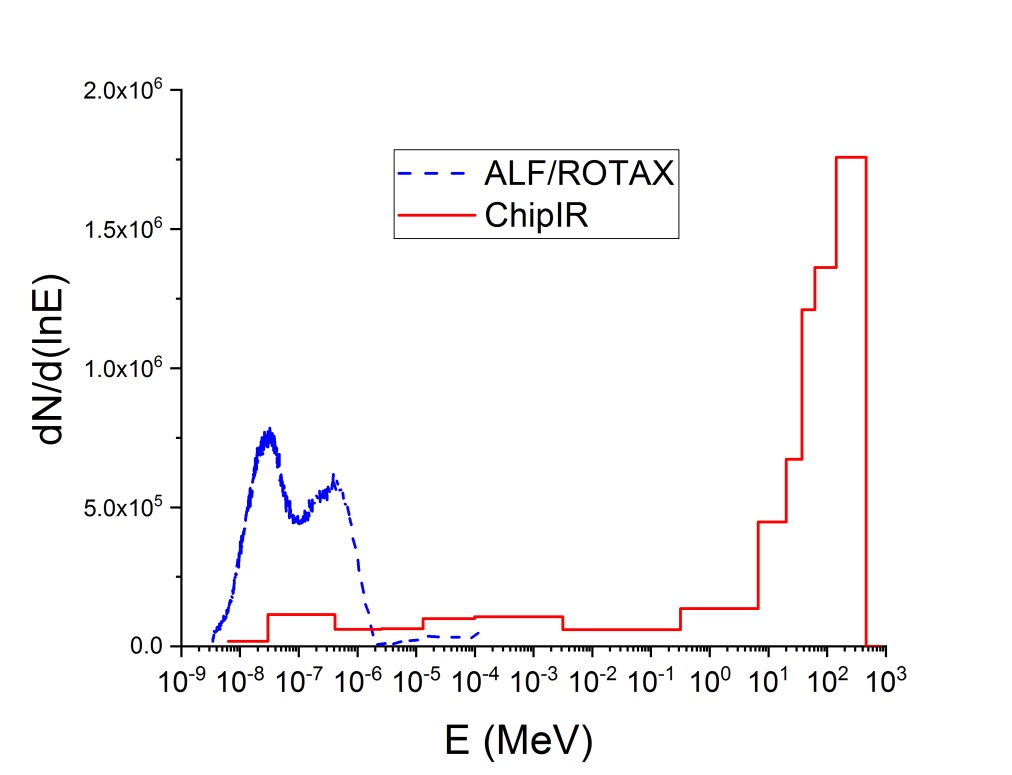
\includegraphics[width=0.35\textwidth]{./figs/rotax-chipir}
\caption{The neutron spectra of the beamlines used for irradiation in lethargy scale.}
\label{rotax_chipir}
\end{figure}


%\subsection{Codes}
\label{subsec_codes}

The set of devices we consider covers a wide range of architectural and computational characteristics. Using the same code for each device would bias the reliability evaluation, in favor of the devices that are more efficient in executing the chosen code. 
To have a fair evaluation, then, we choose for each class of devices the codes that better fit with its computational characteristics. For Xeon Phi and GPUs we chose four codes representative of \textbf{HPC}: MxM, LUD, LavaMD, and HotSpot. We selected three \textbf{heterogeneous} codes specially made to fully utilize the APU architecture: SC, CED, and BFS. Finally, on GPUs and FPGA we tested two \textbf{neural networks} to represent codes that  have a significant impact on self-driven vehicles: YOLO and MNIST. 

\textbf{Matrix Multiplication (MxM)} is representative of highly arithmetic compute-bound codes used in HPC and for features extraction in CNNs. 

\textbf{LUD} is a linear algebra method that calculates solutions for a square system of linear equations.%, representative of highly compute-bound codes~\cite{lava2009}. 

\textbf{LavaMD} simulates particle interactions using Finite Difference Methods. %LavaMD is compute bound, being mostly composed of dot-products. 

\textbf{Hotspot} is representative of stencil solvers, it estimates the processor temperature using an architectural
floor plan and simulated power measurements. 

\textbf{Stream Compaction (SC)} is a memory-bound code used in databases and image processing applications. SC is composed of a data manipulation primitive that removes elements from an array.

\textbf{Canny Edge Detection (CED)} extracts information from images and reduce the amount of data to be processed. CPU and GPU concurrently work on different frames. %The input frames are a subset of the Urban Dataset used for neural networks training \cite{fragkiadaki2012two}. 

\textbf{Breadth First Search (BFS)} is a search in graphs algorithms that performs non-uniform memory access widely used in GPS Navigation Systems. 
%The input graph we select for our evaluation represents the highways of the Great Lakes area in the US \cite{DIMACS} 

\textbf{YOLO} is a Convolution Neural Network (CNN) used for object classification and detection. 

\textbf{MNIST} is a CNN used for classifying handwritten digits. We have tested MNIST only on FPGAs as it is a minimal network that would not exercise sufficient resources on GPUs or Xeon Phis.


%\subsection{Radiation Experiments Setup}
\label{sub_beam_setup}

\begin{figure}[tb]
\centering
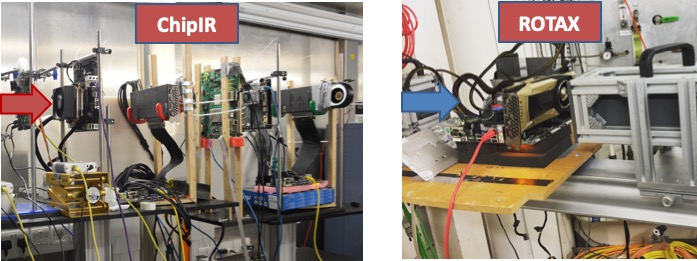
\includegraphics[width=0.80\columnwidth]{./figs/setup}
\caption{Experimental setup in ChipIR and ROTAX. The arrow indicates the direction of the neutron beam.}
\label{rad_setup}
\end{figure}

To evaluate the sensitivity of our devices to high energy and thermal neutrons we exposed the devices on two different beamlines at the ISIS spallation neutron source in the UK: ChipIR for high energy neutrons and ROTAX for thermal neutrons.
ChipIR~\cite{cazzaniga2018progress} is the reference beamline dedicated to the irradiation of microelectronics and it features a high energy neutron spectrum, as similar as possible to the atmospheric one. The flux with neutron energy above 10 MeV is $5.4 \times {10}^6 n/{cm}^2/s$, while the thermal component ($E < 0.5 eV$) is $4 \times {10}^5 n/{cm}^2/s$~\cite{chiesa2018measurement}.
ROTAX~\cite{tietze1989rotax} is a general purpose beamline with a thermal neutron spectrum generating a flux of $2.72\times{10}^6 n/{cm}^2/s$. Here the thermalization is achieved by moderation of the neutrons using liquid methane. 

The spectra of the two beamlines are compared in Figure~\ref{rotax_chipir} on a log-log scale where the fluxes are proportional to the areas under the curves. As Figure~\ref{rotax_chipir} suggests, most neutrons in ROTAX are thermals and most neutron in ChipIR are high energy one.

%To evaluate the sensitivity to thermal and high energy neutrons we align the devices described in Section~\ref{subsec_devices} with the beam, while executing the codes listed in Section~\ref{subsec_codes}. The device output is compared with a pre-computed fault-free copy and any mismatch is marked as an SDC. If the application dies, gets stuck, or the device stops responding we count this as a DUE. Dividing the number of observed errors with the fluence the device has received we can calculate the device sensitivity, expressed as \textbf{cross section} [$cm^2$]. 
%The higher the cross section, the higher the probability for one neutron (either thermal or high energy) to generate an observable error (either SDC or DUE). 
%
%To eliminate any setup-dependent differences between thermal and high energy neutrons, we irradiate the 
%same physical devices executing the codes with the same input vector both in ROTAX and in ChipIR. It is worth noting that, apart from DDR that experienced permanent faults, testing the same device at ROTAX and then at ChipIR (or the other way around) does not influence the measured error rates.
%The only difference between the two experiments is that, thanks to the higher neutron energies, at ChipIR we can align various boards with the beam, as shown in Figure~\ref{rad_setup}. Using a derating factor that takes distance into account we can measure the sensitivity of multiple devices in parallel. In ROTAX, as the irradiate devices stop most of the incoming thermal neutrons, we must test one device at a time. In Figure~\ref{rad_setup} we show the setup for the Titan V evaluation. 

To evaluate the sensitivity to thermal and high energy neutrons we align the devices with the beam, while executing the codes. The device output is compared with a pre-computed fault-free copy and any mismatch is marked as an SDC. If the device stops responding we count a DUE.  To eliminate any setup-dependent differences between thermal and high energy neutrons, we irradiate the same physical devices executing the codes with the same input both in ROTAX and in ChipIR. The only difference between the two experiments is that at ChipIR we can align various boards with the beam, as shown in Figure~\ref{rad_setup}. Using a derating factor that takes distance into account we can measure the sensitivity of multiple devices in parallel. In ROTAX, as the irradiate device block most of the incoming neutrons, we must test one device at a time.
%Due to limitations in the thermal neutrons experiment, we could only test one sample of each device. The high energy neutrons error rate variation among different samples of the same device has already been shown to be low, recent works indicate a variation of about 10\%~\cite{sc2017,Oliveira2017}. 


%\begin{figure}[tb]
%\centering
%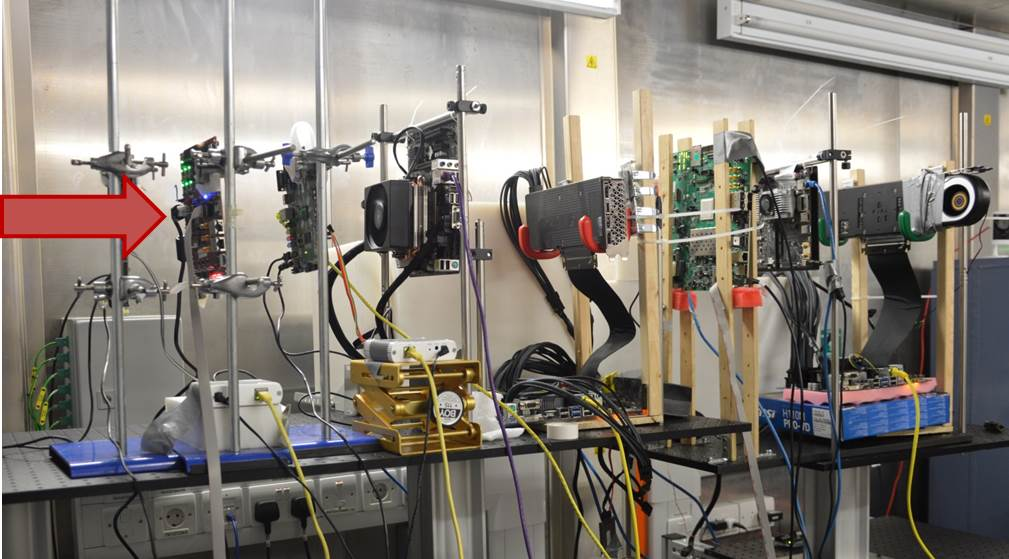
\includegraphics[width=0.90\columnwidth]{./figs/ChipIR_setup}
%\caption{Experimental setup in ChipIR. The arrow indicates the direction of the neutron beam.}
%\label{ChipIR_setup}
%\end{figure}
%
%
%\begin{figure}[tb]
%\centering
%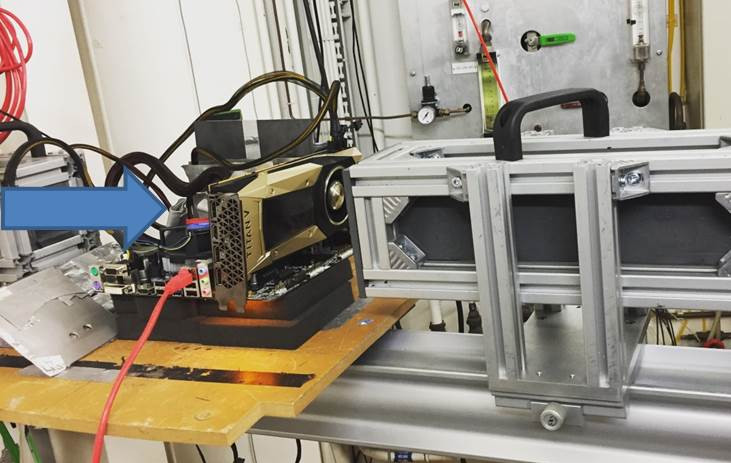
\includegraphics[width=0.9\columnwidth]{./figs/Rotax_setup}
%\caption{Titan X experimental setup in ROTAX. The arrow indicates the direction of the thermal neutron beam.}
%\label{rotax_setup}
%\end{figure}


%\subsection{Thermal Neutrons Detector}
%\label{sub_detector}
%
%
%We have designed and deployed a thermal neutron detector, called Tin-II, to measure the flux of thermal neutrons in different conditions. Ultimately, Tin-II will be used to measure the flux of thermal neutrons inside the data center housing the Trinity supercomputer at LANL. %Tin-II consists of two identical $^{3}He$ cylindrical detectors. The interaction of radiation (neutrons, gammas, betas, etc.) with the detectors triggers a reaction that is amplified, filtered, and counted as an event.
%
%%We calibrated the two detectors for a period of 18 hours to ensure that they have the same detection efficiency. Then, we shielded one of the two cylinders with cadmium. Cadmium effectively blocks thermal neutrons, while being  transparent to  other types of radiation such as high energy neutrons, gammas, betas, etc. As a result, one of the two cylinder (bare detector) detects all radiation reactions, while the other (shielded detector) counts only radiation reactions that are not thermal neutrons. The difference in count rates between these two detectors, multiplied by an efficiency value, reflects the average thermal neutron flux.
%
%Tin-II counted thermal neutron events over the course of several days. To estimate the effect of some of the characteristic materials in modern data centers on the thermal neutron flux, we placed a box containing 2 inches of water close to the detector. The count difference with and without the water, shown in details in Section~\ref{sub_flux}, indicates its influence in the thermal neutrons flux.



%\section{Memories}
\label{sec_memories}


%MAIN INSIGHTS: 
%1 - Figure~\ref{DDRCS}: DDR3 and DDR4 thermal neutrons cross sections. DDR3 and DDR4 have opposite trends for 0-1 and 1-0 bitflips. We have seen both transient, intermittent, permanent fault and SEFIs
%2 - Figure~\ref{DDR}: single and multiple bit distribution shows that ECC could not be sufficient, there is a good amount of multi bit errors induced by neutrons in both DDR3 and DDR4
%3 - Figure~\ref{ddrsc}(next page): We predict the FIT rate of the whole bunch of DDR3 or DDR4 of the 10 fastest supercomputers in the world, considering their memory utilization and their location, simplifying the thermal acceleration factor. We will comment on rainy vs sunny days
%4 - We will compare our estimation with previoulsy published data on DDR FIT rate in some supercomputers

%\begin{figure}[tb]
%\centering
%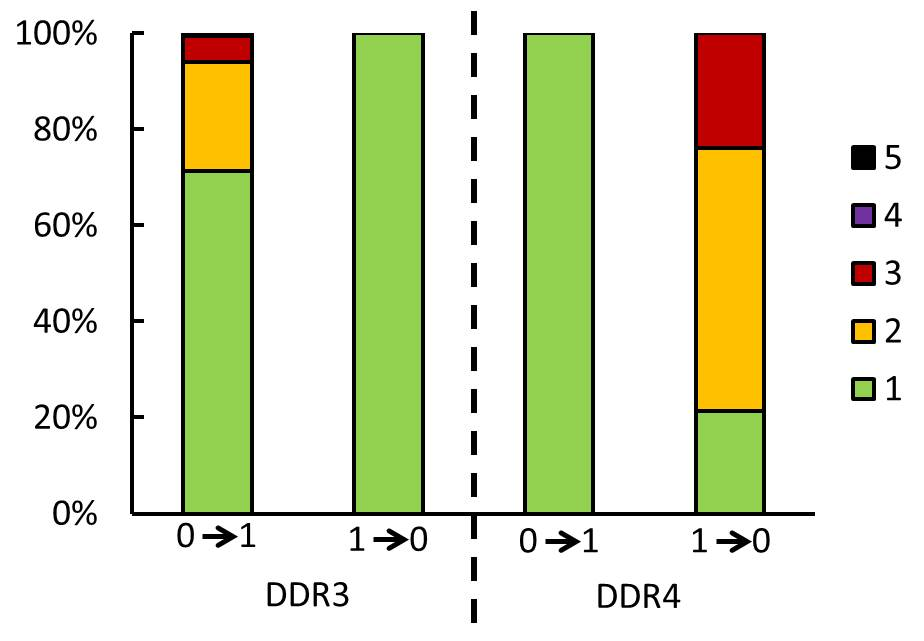
\includegraphics[width=0.9\columnwidth]{./data/plots_final/DDR_errors.jpg}
%\caption{DDR3 and DDR4 Single and Multiple Bit Distribution. }
%\label{DDR}
%\end{figure}


%\begin{figure}[tb]
%\centering
%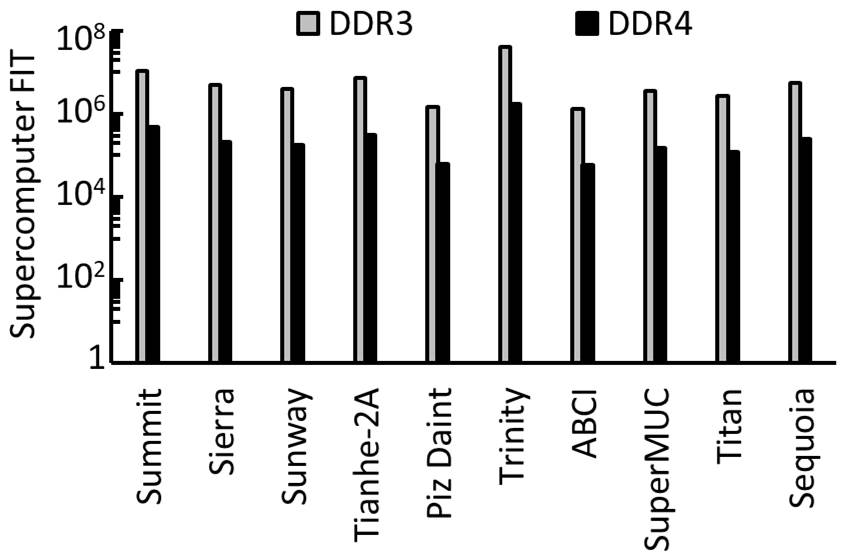
\includegraphics[width=0.9\columnwidth]{./data/plots_final/HPC_FIT.jpg}
%\caption{Predicted DDR3 and DDR4 Thermal FIT rate for the first ten fastest supercomputers from Top500 list.}
%\label{ddrsc}
%\end{figure}

In this section, we present the Double Data Rate (DDR3 and DDR4) Dynamic
Random Access Memories (DRAM) sensitivity to thermal neutrons. Both DDR memories are synchronous DRAM tested without ECC and composed of a single rank x8 memory module. The DDR3 is a 4GB module that operates at 1.5V with a frequency of 1866 MHz and timings 10-11-10. The DDR4 is an 8GB module that operates at 1.2V with a frequency of 2133MHz and timings 13-15-15-28. As vendors are
not explicitly mentioned, cross sections are shown in nominal values. 

We irradiate the devices while performing a continuous read/write \textit{correct loop}: banks are set to 0xFF (or 0x00) and continually read while irradiated with neutrons. When an unexpected value appears, error counters are increased, the corrupted data is downloaded for further analysis, and the memory bank is rewritten. This read/write loop allows differentiating 1-0 and 0-1 bit flips. While Static RAM has a symmetric structure, DDR are likely to be more sensitive to either one of the two possible bit flip directions (one-to-zero and zero-to-one), depending on the cell implementation and on the use of complementary logic.
%The first means the expected value is one and the read value is zero, and the second means the expected value is zero and the read value is one.


The errors are classified into four categories: 
\begin{itemize}[noitemsep]
\item \textbf{Transient error:} a bit flip that does not systematically appear in the following memory read. %That is, incorrect data is read from a memory location but overwritting with correct data. 
%Transient errors in DDR memories have been extensively studied by \cite{baumann2005soft,ziegler1981effect}. 
\item \textbf{Intermittent error:} a memory location returns incorrect values, but not necessarily in consecutive reads. Intermittent errors have been seen in DDR and are dependent on environmental conditions, like temperature~\cite{constantinescu2008intermittent}.
%Abnormal environment conditions, such as elevated temperatures, pollution or cosmic and aplha rays, are responsible for these errors\cite{constantinescu2002impact,sridharan2013feng}. An intermittent error is indicative of device
%damage or malfunction. % In the responsible condition: add cosmic rays and alpha particles.
\item \textbf{Permanent error:} a memory location consistently returns an incorrect value (stuck-at). Permanent errors are caused by Displacement Damage (the neutron dislocates atoms in the transistor) and can possibly be repaired with annealing (i.e., heating the device)~\cite{quinnDDR,srour2003}.
%\cite{constantinescu2003trends}. 

\item \textbf{Single Event Functional Interrupt (SEFI):}  a large portion of the memory array return incorrect values, likely caused by an error in the DDR control logic circuits. Further reads/writes will return correct values~\cite{electronic1996test}.

\end{itemize}

\begin{figure}[tb]
\centering
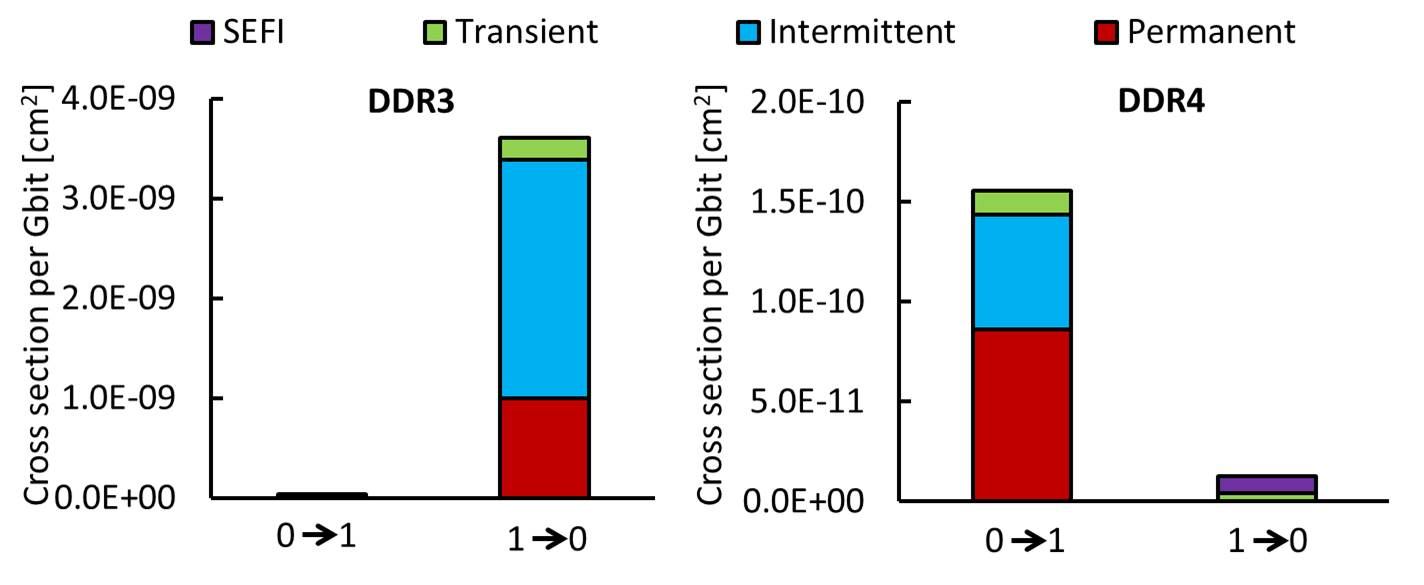
\includegraphics[width=1.00\columnwidth]{./data/plots_final/cs_DDR.jpg}
\caption{DDR3 and DDR4 thermal neutrons cross sections.}
\label{DDRCS}
\end{figure}

Figure~\ref{DDRCS} shows the thermal neutrons cross section per GBit for DDR3 and DDR4. We do not report high energy neutron data since after few minutes of irradiation at ChipIR both DDR3 and DDR4 experienced a high number of permanent faults, impeding further data collection. However, the sensitivity of DDR memories to high energy neutrons has been extensively studied, and experimental data can be found in~\cite{constantinescu2002impact,sridharan2013feng,quinnDDR,guertin2017}.

Figure~\ref{DDRCS} highlights that the DDR4 memory cross section is approximately one order of magnitude lower than the DDR3 one, showing significant reliability improvements probably resulting from new manufacturing processes as well as transistor placement enhancement. We also observe in Figure~\ref{DDRCS} that more than 95\% of all the errors are in one of the two possible bit flip direction, one-to-zero for DDR3 and zero-to-one for DDR4. The opposite direction for DDR3 and DDR4 suggests that one device is manufactured with complementary logic. 
Another interesting point our data highlights is the proportion of each error category changes from DDR3 to DDR4. Permanent errors are more than 50\% of all observed errors in DDR4, while on DDR3 only less than 30\% of errors are permanent. It is also worth noting that both technologies present SEFI errors during the experiments. That is, an impinging particle on both DDR memory control circuits tend to incite similar malfunctioning behaviors.

Finally, all the observed transient and intermittent errors were single bit
flip. This is a promising result, as SECDED ECC is shown to be sufficient to
corrects most thermal neutrons induced errors~\cite{sridharan2012study}. On the contrary, in a SEFI error multiple corrupted bits were observed.


%DDR4 memory errors are less likely to happen but with a greater impact to normal operation;

%Despite presenting better general results, DDR4 memories are more susceptible to radiation-induced permanent errors. That is, DDR4 memories errors generate more critical output corruption as the fault persist on time.
%Intermittent radiation-induced memory errors affect in a greater way the DDR3 device. A possible reason for that is the diminution of voltage operation introduced by DDR4 technology.
% Transient errors appear to remain constant between both tested devices.

%An important result observed is that both technologies present SEFIs errors during the experiments. This is, an impinging particle on both DDR memory control circuits tend to incite similar malfunctioning behaviours.   

 %As SEFI is caused by bit flip in memory control circuits, corrupt data may occur in random and multiple positions.


%Falar sobre erros que não sçao SEFIS então o ECC consegue corregir tudos os erros. Nos sefis não tem o que fazer porque são erros na logica de controle



\begin{figure*}[tbh]
	\centering
	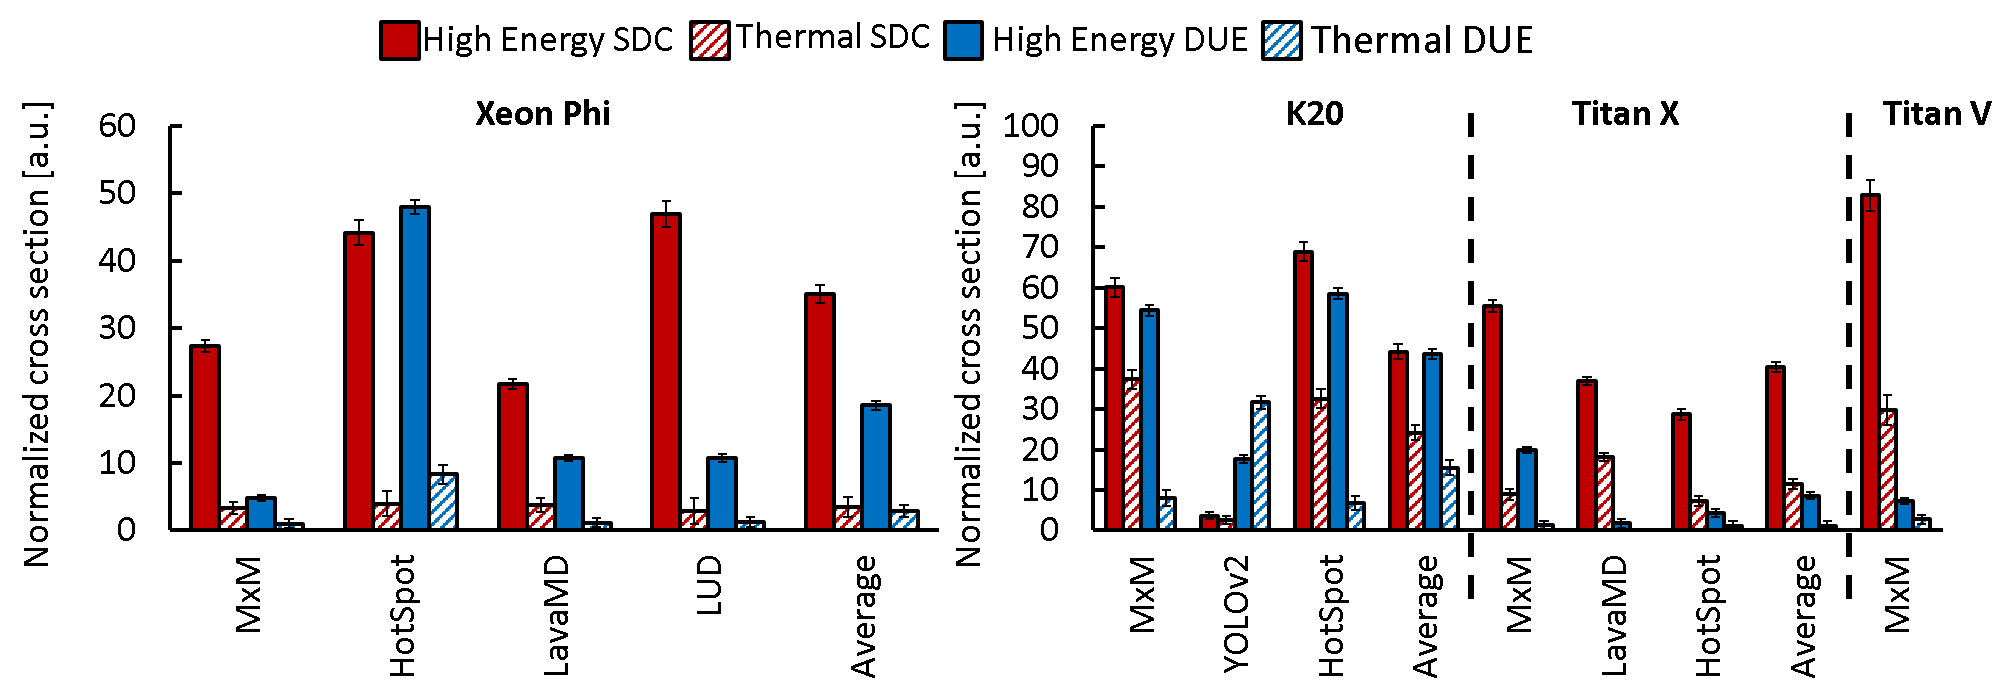
\includegraphics[width=0.79\textwidth]{./data/plots_final/cs_xeon_gpus_avg.png}
	\caption{High energy and thermal neutrons normalized cross sections for Xeon Phi and GPUs.}
	\label{cs_xeon_gpus}
\end{figure*}

\begin{figure*}[th]
	\centering
	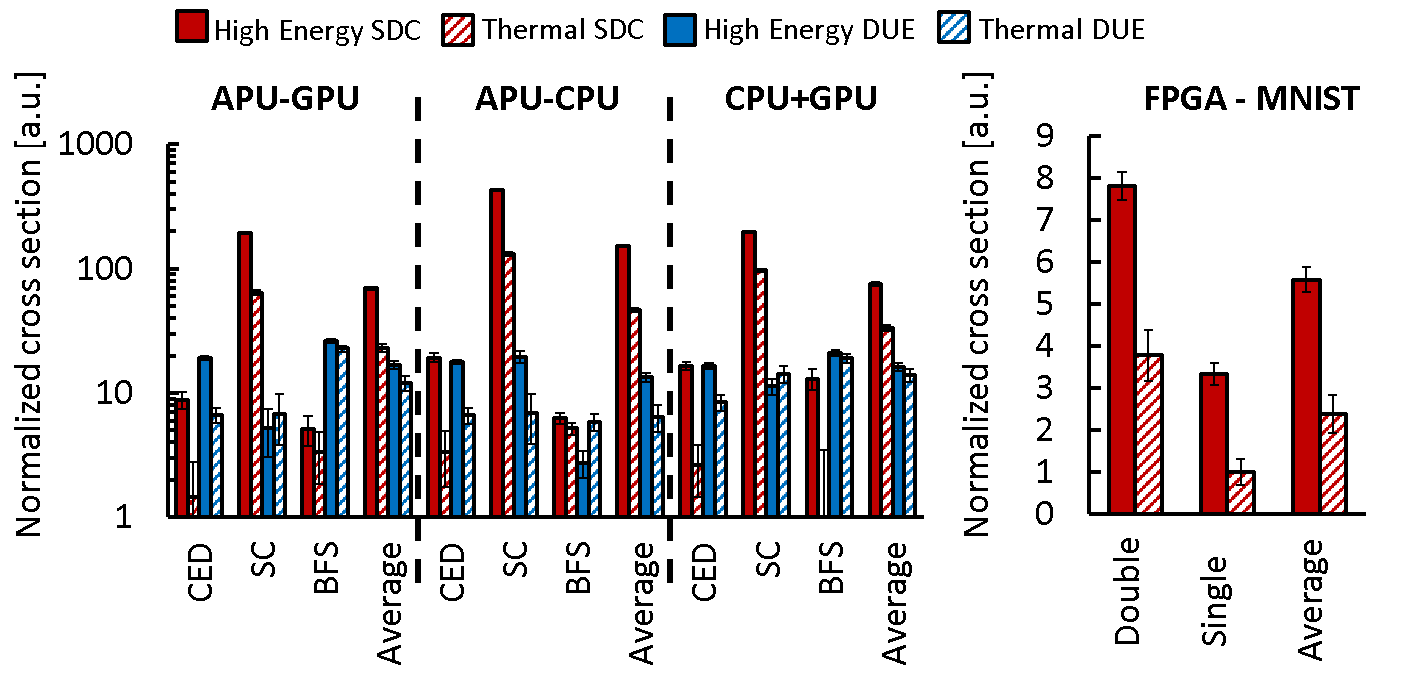
\includegraphics[width=0.69\textwidth]{./data/plots_final/cs_APU_FPGA_avg.png}
	\caption{High energy and thermal neutrons normalized cross sections for AMD APU and FPGA.}
	\label{cs_apu_fpga}
\end{figure*}

\section{Cross Section Results}
\label{sec_results}

In this section, we compare the cross section measured at ChipIR and ROTAX for the tested devices and codes with the methodology described in Section~\ref{sub_beam_setup}. We emphasize that we used exactly the same device and setup for both ChipIR and ROTAX experiments. %Due to beam time limitations (mainly at ROTAX as we must test only one device at a time) we could not test all the benchmarks in each device.
%Recall that a higher cross section indicates a higher probability of a single (high energy or thermal) neutron inducing faults. To evaluate the impact of thermal vs. high energy neutrons on the device error rate we need to consider the natural background flux, which is done in Section~\ref{sec_fit}.
As we show, the cross section to thermal neutrons is far from being negligible, indicating the presence of $^{10}B$ in the silicon doping. Reported data have been normalized to the lowest cross section for each vendor to prevent the leakage of business-sensitive data while allowing a direct comparison between codes and devices of the same vendor. We also report error bars considering Poisson's 95\% confidence interval.

Figure~\ref{cs_xeon_gpus} shows the \textbf{Xeon Phi} SDC and DUE cross sections for high energy and thermal neutrons. On  average the thermal neutrons cross section is much lower ($1/20$) than the high energy neutrons' one, for both SDC and DUE.
This low sensitivity to thermal neutrons is a sign that either little boron is used in the production of Xeon Phi.
%HotSpot is the most sensitive code for both
%SDCs and DUEs. HotSpot is especially sensitive to DUEs, with a cross section
%more than $2\times$ higher than the average for both high energy and thermal
%neutrons. HotSpot, in contrast to the other codes, uses a high number of
%control flow statements and has low arithmetic intensity, increasing the
%sensitivity to DUEs. 


For SDCs, the high energy neutron cross sections vary significantly depending on the code being executed (more than 2x across codes), which is in accordance with previous work~\cite{sc2017, fratin2018DSN}. The SDC cross sections for thermal neutrons, however, have a very low variation between codes (less than 20\%) which may be an artifact of the low number of SDCs observed. This result suggests there is a negligible sensitivity to thermals in the  chip resources that are responsible for the variation between error rates in the high energy SDC results.
DUEs, on the other hand, have a similar trend for high energy and thermal neutrons. %DUE faults induced by thermal neutrons seem to have similar effects to DUE faults induced by high energy neutrons. 

Figure~\ref{cs_xeon_gpus} shows the sensitivity of \textbf{NVIDIA GPUs} to thermal and high energy neutrons.
For the K20, on the average, both the SDCs and DUEs thermal cross sections are very high, being 60\% and 50\% of the high energy neutrons ones. This indicates the presence of a significant amount of $^{10}B$ in the manufacturing process. The thermal neutrons SDC cross section trend across codes is also similar to the high energy neutrons one, in the sense that the code with the largest thermal neutrons cross section (i.e., HotSpot) is also the code with the largest high energy neutron cross section. This suggests that $^{10}B$ is present in the computing resources and memory of these devices, and that the fault locations are similar for both kind of neutrons. 
%
It is also interesting to notice that YOLOv2 is the only code for which DUEs are more likely than SDCs, for both kind of neutrons. This result follows previous work that shows low SDC sensitivity in CNN based object detection~\cite{ffsantos2018}. %As shown in Figure~\ref{cs_xeon_gpus}, YOLOv2 DUE cross section for thermal neutrons is more than 50\% higher than the DUE cross section for high energy neutrons and more than $2\times$ higher than the average of all K20 codes. This cross section indicates that the reliability for YOLOv2 in environments where thermal neutron flux is significant will be much worse than expected, especially for a safety-critical application like self-driven cars.

For Titan X and Titan V, on the average, the thermal neutron cross section is an order of magnitude lower than the high energy one. The impact of thermal neutrons is lower for the newest GPUs than on the mature K20. This may imply that
FinFET based GPUs are less susceptible to thermal neutrons than CMOS GPUs (K20 is built using CMOS planar transistors, Titan X and Titan V using FinFET). However, for the MxM tests, Titan V
($12nm$) shows an almost doubled thermal neutron SDC cross section compared to
the Titan X ($16nm$). Unfortunately, we were not able to test more codes on
the Titan V to confirm if the increased thermal neutron cross section is intrinsic of smaller FinFET technologies.


The \textbf{AMD APU} cross sections are shown in Figure~\ref{cs_apu_fpga}. As described in Section~\ref{subsec_devices}, the APU embeds a GPU and a CPU. We test the three heterogeneous codes described in Section~\ref{subsec_codes} (CED, SC, and BFS) as executed on the GPU only, on the CPU only, and distributing concurrently 50\% of the workload to the CPU and 50\% to the GPU (CPU+GPU).

The APU-GPU, APU-CPU, and CPU+GPU SDC cross section for both thermals and high energy neutrons vary of more than an order of magnitude, forcing the use of logarithmic scale for APU data in Figure~\ref{cs_apu_fpga}. The reported data shows that, on the average, the thermal neutrons cross section is  between $1/4$ and $1/5$ the high energy neutron's, for CPU, GPU, and CPU+GPU.
All APU configurations, on average, are more sensitive to SDCs than DUEs. It is also worth noting that the APU-CPU has, on average, a higher SDC sensitivity than APU-GPU. This is in accordance with previous work that shows a much lower probability for a fault in the AMD GPU to impact the application output than a fault in the CPU~\cite{Jeon2013ArchitecturalVM}. %Additionally, in the APU, the GPU has a significantly smaller physical area than the CPU which reduces the probability of a neutron striking it and causing corruption.

%A specific result to highlight is that SC code, which is the only memory-bound
%code of the three we test on the APU, has an SDC sensitivity to both high energy and thermal
%neutron extremely high when compared to others. As already shown, when the device is in idle waiting for data to be fetch from memory, registers and caches are exposed to radiation and store critical data~\cite{fratin2018DSN}. Moreover, as observed for the Xeon Phi,
%the DUE cross section variation across different codes is much smaller than SDC variation. 
%Finally, BFS has a particularly high DUEs sensitivity when
%the GPU is involved in computation (APU-GPU and CPU+GPU). This DUE increase is likely caused by the
%much higher stress in the CPU-GPU synchronization that BFS imposes by launching several GPU kernels~(refer to section~\ref{subsec_codes}).

Figure~\ref{cs_apu_fpga} shows \textbf{Xilinx FPGA} SDC cross section when executing the MNIST CNN. It is worth noting that neutron-induced errors in the configuration memory of SRAM FPGAs have a \textit{persistent} effect, in the sense that a corruption changes the implemented circuit until a new bitstream is loaded in the device. The observation of an error at the FPGA output indicates that the bitstream has probably been corrupted. 
We reprogram the FPGA at each observed output error to avoid the collection of a stream of corrupted data, making the observation of DUEs very rare. In fact, as FPGA executes operation without any operating system, interfaces, or control-flow involved, a considerable amount of errors would need to accumulate in the configuration memory to have the circuit functionality compromised. We never observed a DUE in FPGAs during our experimental campaign.

We have tested two different versions of the neural network, one using double and the other using single precision floating-point arithmetic. When comparing the high energy and thermal neutrons cross sections for the two configurations, we can clearly perceive that the Xilinx FPGA is more sensitive to high energy neutrons. However, the thermal neutrons cross section is far from being negligible.

The double precision version takes about twice as many resources to be implemented in the FPGA. As the neutrons cross section is directly related to the circuit's area, the cross section is expected to be higher for the double version of MNIST. Experimental results for both high energy and thermal neutrons confirm this intuition. The thermal neutrons cross section for the double version is particularly higher than the single one, being almost four times larger.

\begin{figure*}[!tb]
    \centering
    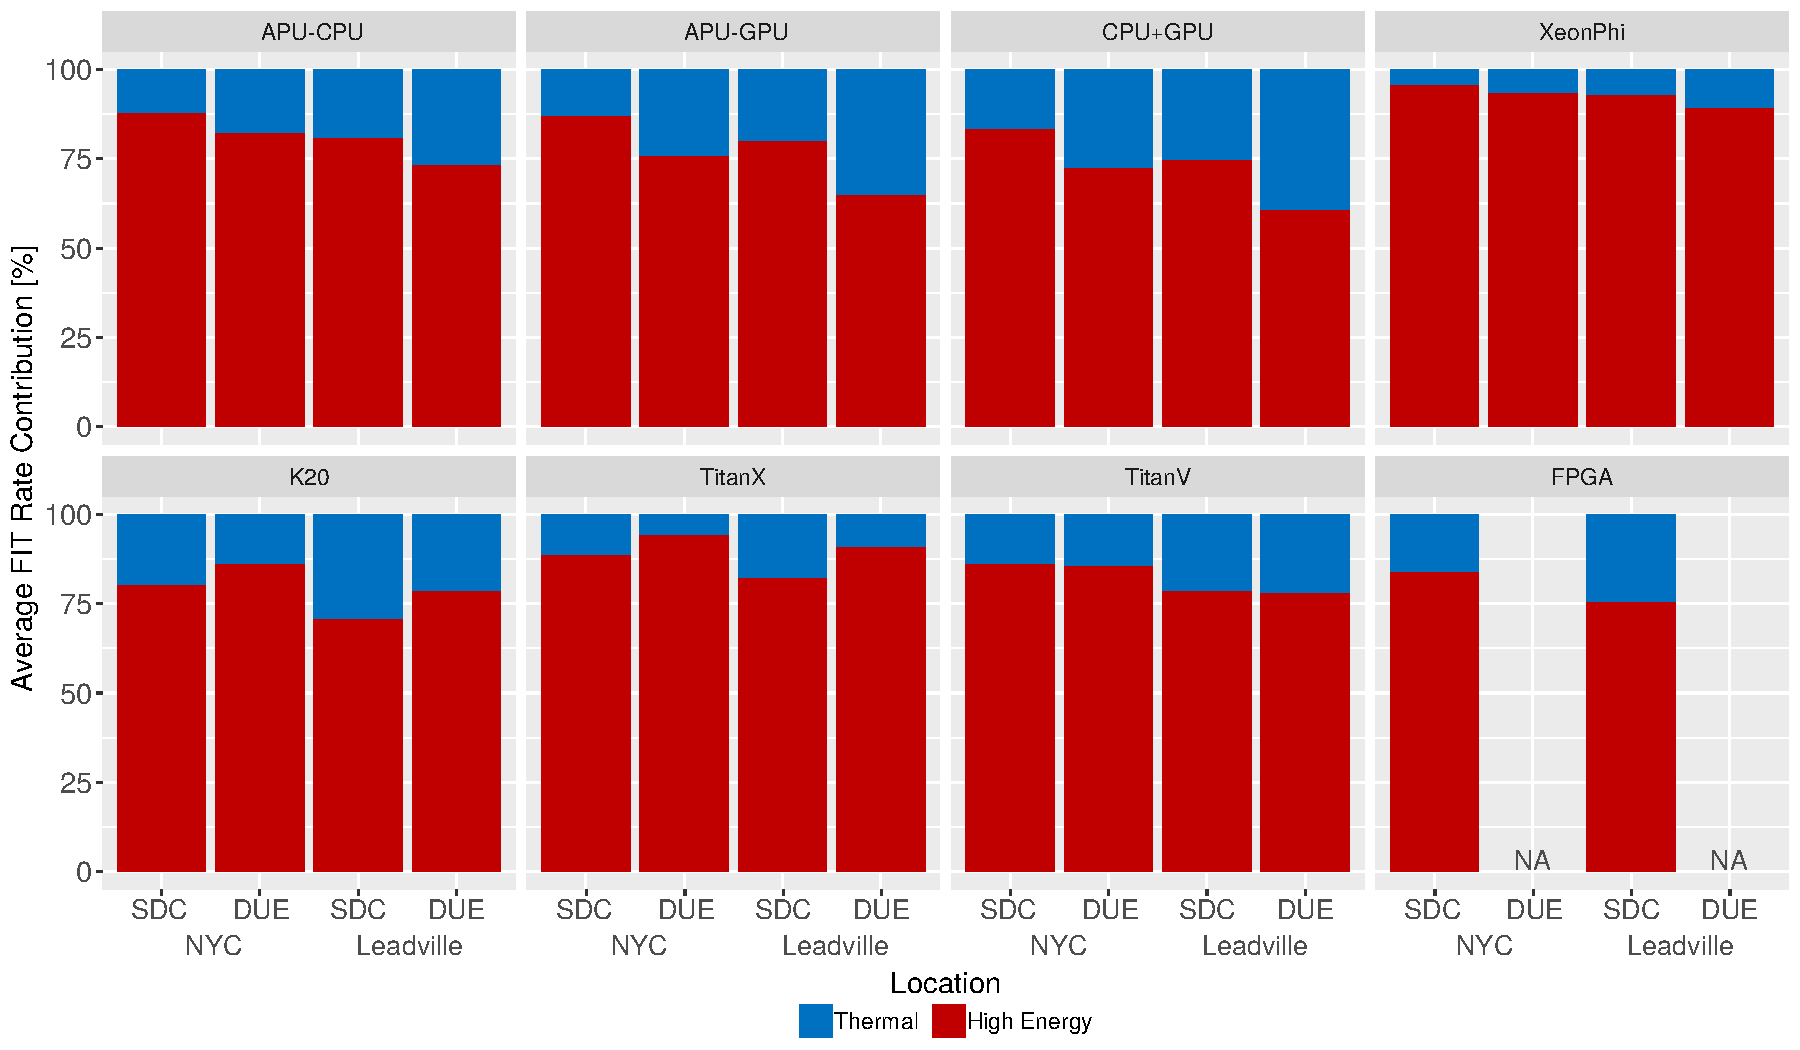
\includegraphics[width=0.82\textwidth]{figs/FIT-rates-all-devices.pdf}
    \caption{Percentage of total FIT rate due to high energy and thermal neutrons. All tested parts except Xeon Phi show significant errors due to $^{10}B$ levels.}
    \label{fig_fitpercents}
\end{figure*}

Our results show that different codes executed on the same device can have very different high energy vs thermal neutrons sensitivities. 
The physical interaction of a thermal neutron and, consequently, the resulting fault model (i.e., the way the physical fault is manifested at circuit level) and the impact on the code execution is highly different from the high energy neutron. 
%High energy neutrons can interact with any atom in the chip or package material, triggering a reaction that may potentially reach a transistor's vulnerable area. The fault can happen some distance from the high energy neutron impact, and the particles resulting from the interaction can travel in different directions~\cite{Baumann2005}. Thermal neutrons, on the other hand, interacting only with  $^{10}B$, produce an alpha particle and lithium recoil that have very short ranges. When a thermal neutron is absorbed in virtually all other materials used in semiconductor manufacturing, the resulting nuclei typically only produces  gamma rays, which do not produce bit flips. 
Software fault-injection can emulate predefined fault models and study their effects, but cannot be used to study the fault manifestation nor to define different fault models. One way to investigate the different fault models would be to simulate the physical implementation of a transistor in a given technology and observe the effect of neutron strikes at different energies~\cite{Dodd2005}. However, transistor implementation details are not available for COTS devices, which makes the comparison of the beam experiment cross sections of various codes the only possible way to highlight code-dependent thermal vs high energy neutrons induced error rates.


%\begin{figure}[tb] 
%\centering
%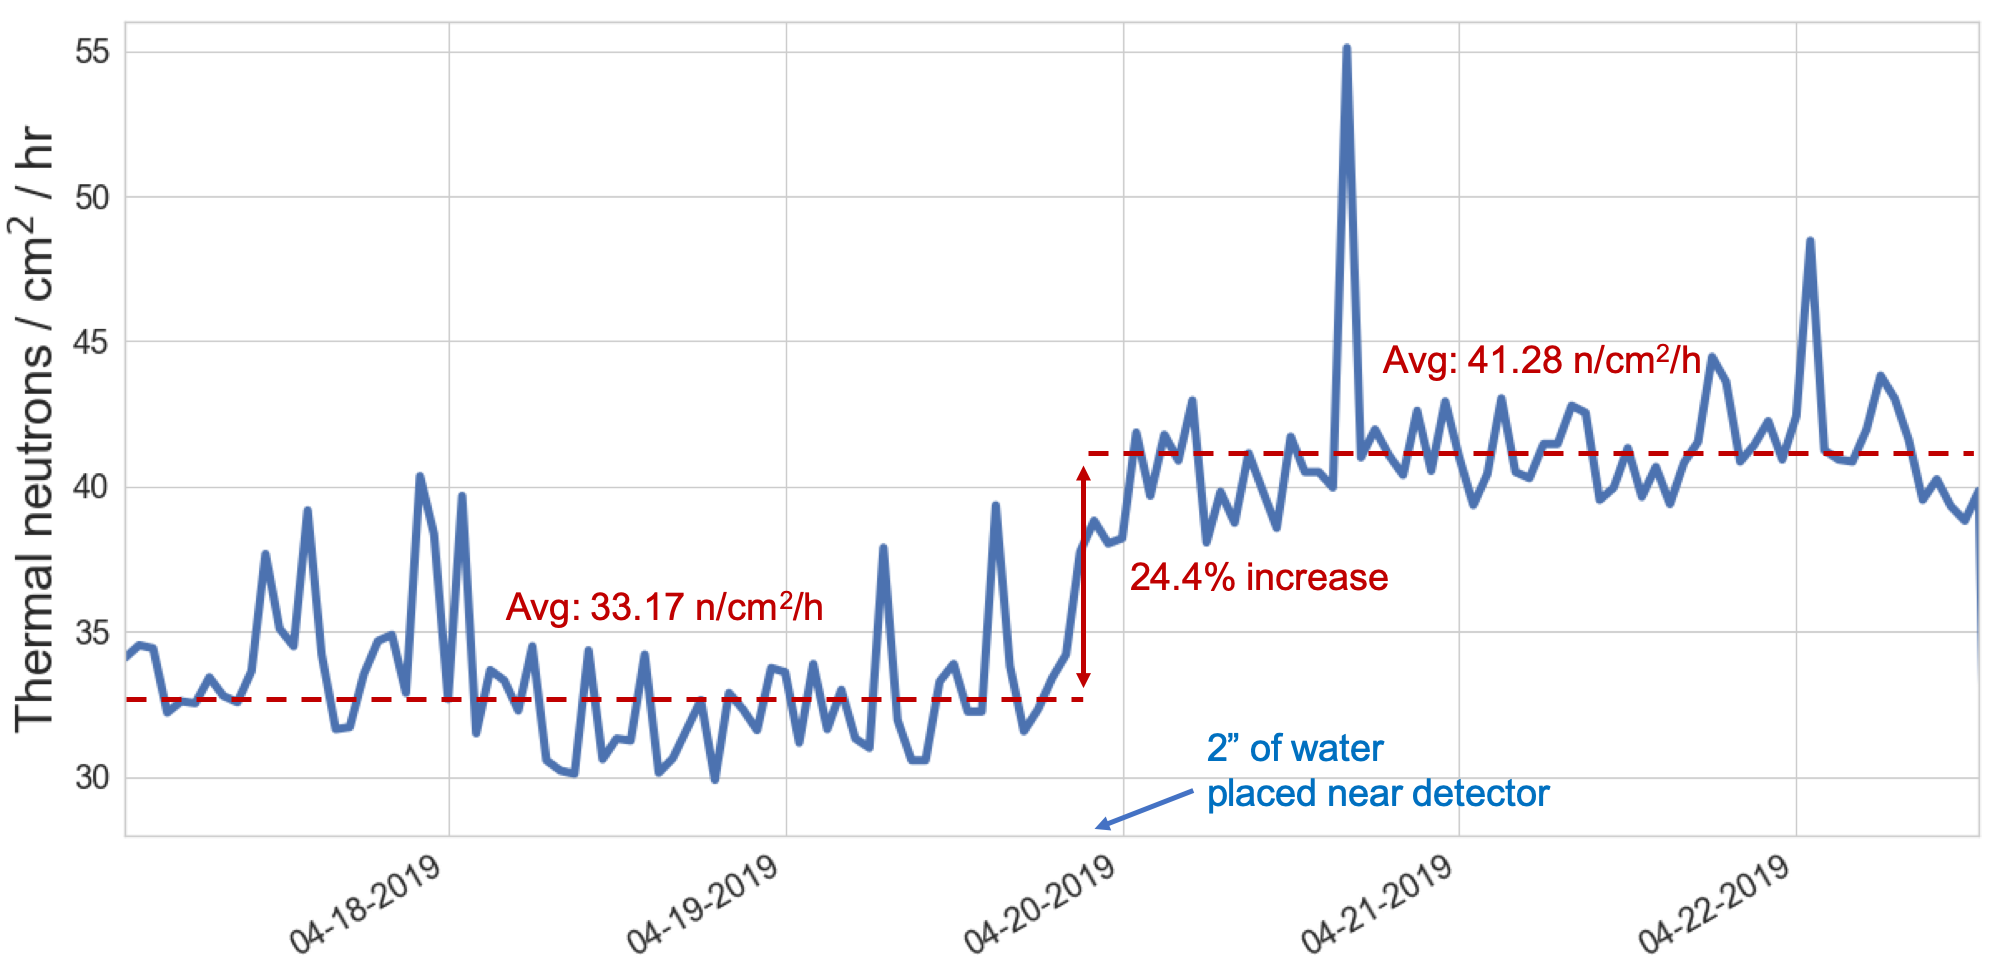
\includegraphics[width=0.82\columnwidth]{./figs/turkeypan_PR}
%\caption{Tin-II thermal neutron detector measurements with two inches of water placed over detector on $20^{th}$ April 2019.}
%\label{turkeypan}
%\end{figure}

%\begin{figure*}[!tb]
%    \centering
%    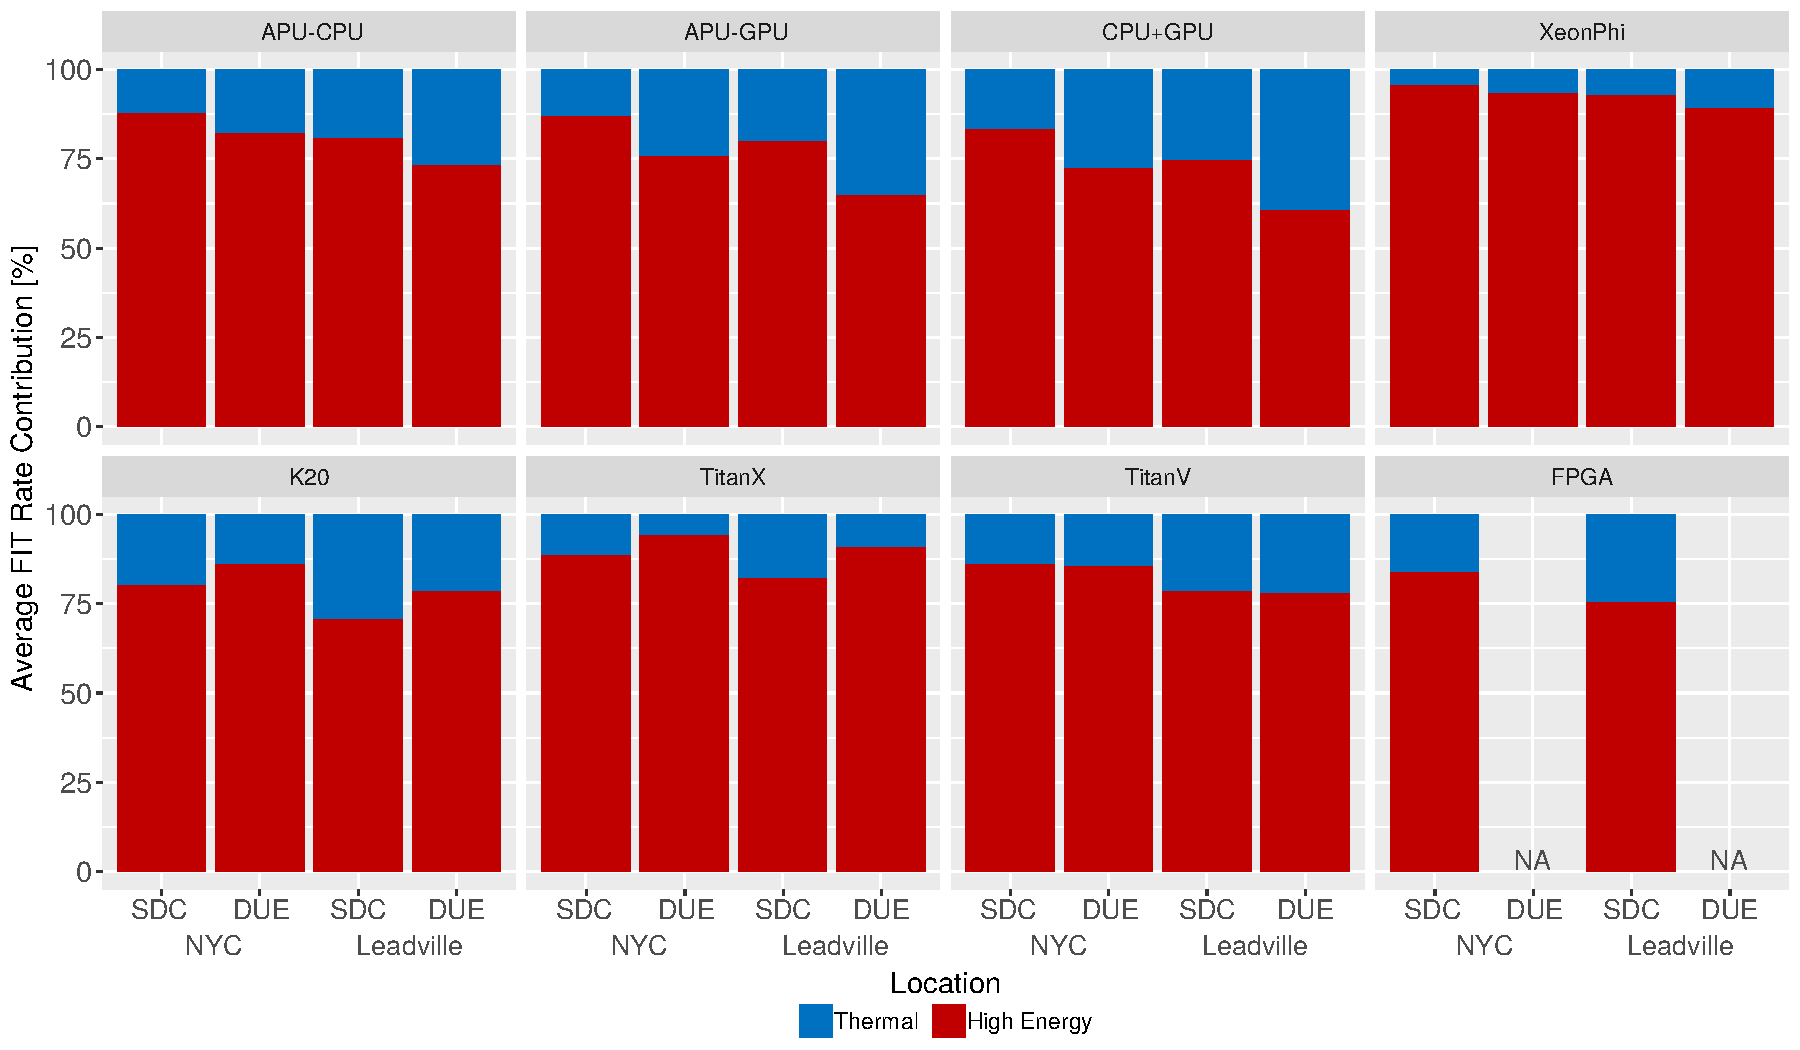
\includegraphics[width=0.85\textwidth]{figs/FIT-rates-all-devices.pdf}
%    \caption{Percentage of total FIT rate due to high energy and thermal neutrons. All tested parts except Xeon Phi show significant errors due to $^{10}B$ levels.}
%    \label{fig_fitpercents}
%\end{figure*}


\section{FIT Rate Analysis}
\label{sec_fit}


The cross sections reported and discussed in Section~\ref{sec_results}, represent the device's sensitivity to thermal or high energy neutrons. To have an understanding of the impact of thermal and high energy neutrons in the device error rate, we need to consider the natural background radiation fluxes of each. FIT rates can then be calculated by multiplying the experimentally measured cross sections by the neutron fluxes. We only show in percentages the contribution of thermal and high energy neutrons to the device's FIT rates to avoid the leakage of business sensitive data. This information allows us to evaluate how much thermal neutrons increases the FIT of each device. This also tells us how much the FIT rate of each device is underestimated if thermal neutrons are not considered.


%\subsection{Thermal Neutrons Flux}
\label{sub_flux}

The flux for high energy (fast) neutrons in the atmosphere can be precisely estimated considering the
altitude, longitude, latitude, and solar activity. However, the environment and the materials that surround a device significantly impact neutron flux and energy. 
%Materials such 
%as concrete and water scatter neutrons which lose energy with each interaction.
For instance, during thunderstorms the rain droplets act as moderators slowing high
energy neutrons into lower energy ones. The thermal neutron flux, as measured
in~\cite{ziegler2003}, can be as much as $2\times$ higher during a rain storm than on a sunny day. Thermal neutron rates may be as much as 20\% higher over a large slab of concrete such as in a parking lot or the concrete floor of a machine room. 
Water cooling systems can also have the side effect of significantly 
increasing the proportion of thermal neutrons that strike a device.

%In order to  empirically measure the impact of materials in the thermal neutron flux in a data center, we placed the Tin-II detector (details in Section~\ref{sub_detector}) in a building similar to the one containing the Trinity supercomputer. We collected data over the course of several days, then placed 2 inches of water in a box over the detector starting on $20^{th}$ April 2019. Figure~\ref{turkeypan} shows that when water is placed over the detector the thermal neutron counts abruptly increase of about 24\%. This increase shows that the presence of water in the cooling system can significantly increase the rates of thermal neutrons in a system, which in turn will increase the rates in the devices sensitive to those neutrons as seen in section~\ref{sec_results}. 

%Furthermore, to confirm the statistical significance of the thermal neutron flux calculation in our Tin-II experiments, Figure~\ref{tin2hist} displays the count rate of the thermal neutrons over time for our detector, the density function uses a Gaussian kernel density estimate. As can be seen, there are two main groupings of the data. The bimodal distribution is due to the water being placed over the detector on $20^{th}$ April 2019.

%\begin{figure}[tb]
%\centering
%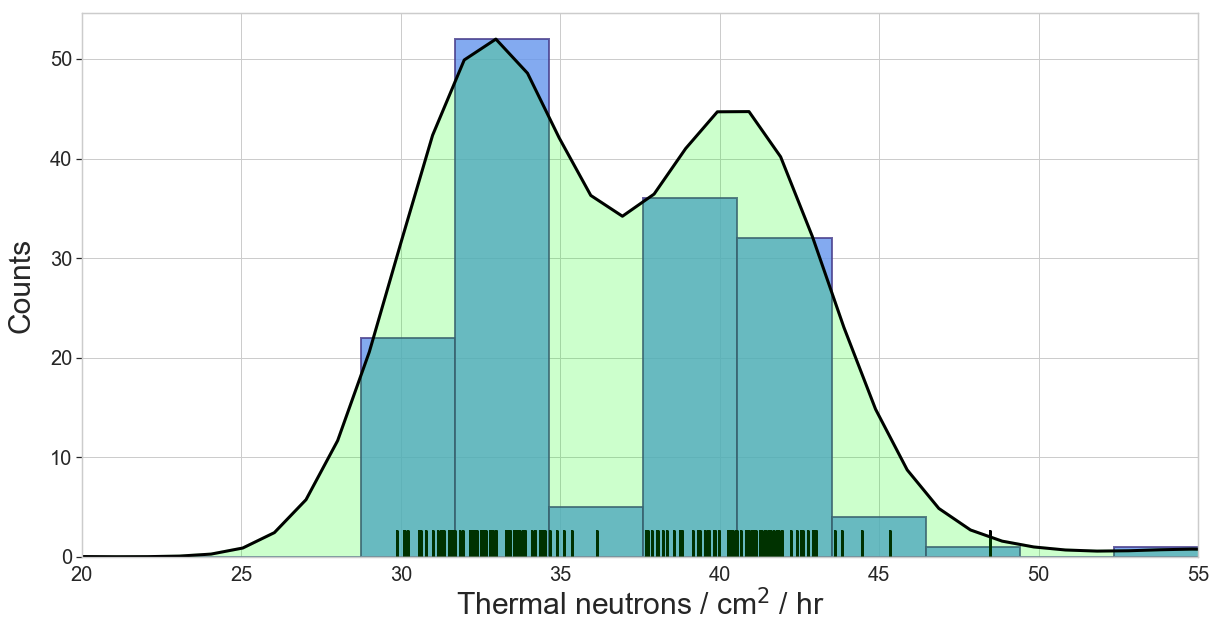
\includegraphics[width=1.00\columnwidth]{./figs/kde_bimodal_with_histogram}
%\caption{Tin-II thermal neutrons count rate. The bimodal distribution shows the influence of water placed above the detector.}
%\label{tin2hist}
%\end{figure}



%The shape and placement of a water cooling system can  impact the way thermal neutrons are produced. The LANL's Trinity supercomputer's water cooling pipes are below the machine which sits several feet above a concrete slab, whereas ORNL's Summit machine sits directly on a concrete slab with water cooling pipes running overhead. Both of these machines have liquid cooling radiators in the racks. Based on physical considerations, we believe the final flux for most liquid-cooled machines will be elevated. 


These same considerations exist when trying to understand the thermal neutron component of faults in autonomous vehicles. The road material, concrete or asphalt, the vehicle is driving on makes a difference, as does the weather, and the type and volume of fuel the vehicle uses. In addition, the number of passengers will change the thermal neutron flux, as humans are primarily composed of water  which makes us excellent neutron moderators. 

%\subsection{High Energy vs Thermal Neutrons FIT}


Figure~\ref{fig_fitpercents} shows the percentage of the total FIT rates due to high energy and thermal neutrons. These calculations use measured values of neutrons at sea level (NYC) and in Leadville, CO (10,151 ft in altitude). The thermal rates used have been adjusted to compensate for back scattered neutrons from a concrete slab, an overall increase of 44\% in the thermal flux. Note that on a rainy day the thermal flux may be as much as doubled over the rates used in this graph and the corresponding FIT rate on those days will increase in a corresponding way~\cite{ziegler2003}.

Xeon Phi processors, 
 as stated in Section~\ref{sec_results}, have a low sensitivity to thermals, which is a symptom of the use of either depleted boron or a reduction in boron usage. 
 Thus, the thermals FIT rate seen in figure~\ref{fig_fitpercents} is a relatively small percentage of the overall FIT rate (from 4.2\% at NYC SDC up to 10.6\% for Leadville DUE).
The other tested devices, especially the K20 and CPU+GPU devices, have thermal FIT rates comparable to the FIT rates from high energy neutrons. At Leadville, K20 has 29\% of the SDC FIT rate caused by thermal neutrons while APU CPU+GPU has 39\% of DUEs caused by thermal neutrons.

%\subsection{Discussion}


Figure~\ref{fig_fitpercents} shows that if thermal neutrons contribution to the device error rate is not considered both the DUE and SDC FIT rates could be significantly underestimated, posing unconsidered risks to a safety critical application or reducing the HPC server productivity unexpectedly. 
Of particular interest in Figure~\ref{fig_fitpercents} is the relatively high percentage of
faults that result in Silent Data Corruption (SDC) on several of the tested devices. In general, HPC systems are designed and engineered to maintain SDC rates low and manageable, where corrupted calculations are rare and often noticeable to users. However, anything that increases the SDC rate is always concerning. In safety critical applications, SDCs should be strictly avoided as they could put the system in unexpected states, and they could potentially lead to unpredictable actions.

The elevated DUE rates are also of concern as they result in a system crash and loss of some portion of a calculation's run time. 
It is worth noting that even with thin layers of shielding, embedded devices in vehicles can suffer from a much higher thermal flux than the one considered in Figure~\ref{fig_fitpercents} due to moderation and reflection from the surrounding materials.%~\cite{leo2012techniques}.

%Our analysis shows that thermal neutrons are a threat for the reliability of supercomputers and safety critical applications that rely on COTS HPC devices. While the benefits in terms of cost, performances, and efficiency of COTS devices are not in question, their utilization in applications for which reliability is a concern must be coupled with a careful reliability evaluation that considers the impact of thermal neutrons. As the amount of $^{10}B$ in the manufacturing process is not publicly available, radiation experiments are one of the few ways to evaluate the sensitivity of a COTS device to thermal neutrons. %Moreover, as the thermal neutron flux strongly depends on environmental conditions, the device error rate varies significantly when conditions change. Therefore it is critical to consider the realistic conditions in which the device will operate and estimate the correspondent thermal neutrons flux. These conditions have a direct impact on HPC applications. For instance, when supercomputer time is allocated, the checkpoint frequency may need to  consider weather conditions.
%Dissimilarly to high-energy neutrons, thermal neutrons flux can be effectively reduced shielding the device with thin layers of cadmium or some inches of boron plastic. Unfortunately, cadmium is highly toxic and should not be heated, so it should not be placed in the proximity of an HPC device or of a cooling system, and boron plastic also thermally isolate the device, so it is impractical to be used as a shield between the cooling system (one of the most efficient sources of thermal neutrons) and the device. 


\section{Conclusions}
\label{sec_conclusion}

In this paper we have experimentally investigate the differences between high
energy and thermal neutron induced error rates in modern HPC devices. %While purifying the Silicon dopant to remove $^{10}B$ would make  devices immune to thermal neutrons, most COTS still use natural Boron. 
By irradiating devices  with high energy and thermal neutrons while executing representative applications,  we have demonstrated that thermals significantly impact device reliability.
We have demonstrated that the impact of high energy and thermal neutrons depends not only on the specifics of the hardware, but also on the executed code. The impinging neutron energy has more or less effect depending on how the code accesses memory and executes instructions. 

We have also shown that the FIT rates can vary based on the physical layout of the machine room in which a system resides and variations such as weather conditions external to the building. 
%We have also evaluate the FIT rates on different scenarios, considering concrete walls %attenuation and weather conditions. 
%When it is raining, the thermal-induced error rate significantly increases. 
%
The reported data attests the importance of thermal neutron reliability
evaluation, which can significantly raise the total device error rate. %As a future work, we plan to irradiate with thermal and high energy neutrons specific resources or components to deeply investigate different fault models. We also plan a thorough and sophisticated modeling of one or more  data centers as well as the effects of different cooling regimes.




\bibliographystyle{IEEEtran}
\bibliography{ref}


\end{document}


